\documentclass[12pt,a4paper]{article}

\usepackage[utf8]{inputenc}
\usepackage[spanish]{babel}
\usepackage{graphicx}
\usepackage{booktabs}
\usepackage{amsmath}
\usepackage{float}
\usepackage{hyperref}
\usepackage{geometry}
\geometry{a4paper, margin=2.54cm}
\usepackage{setspace}
\spacing{1.5}

\title{\textbf{Comparación experimental del modelo Manager--Worker usando hilos de plataforma vs hilos virtuales (Java 21)}}
\author{Sergio Gil Guerrero García \\ Examen General de Conocimiento para Obtener el Grado de Maestría}
\date{Fecha de entrega: 23 de febrero}

\begin{document}

\maketitle

\begin{abstract}
El presente documento expone el diseño, desarrollo y resultados de un experimento controlado destinado a evaluar el desempeño de la concurrencia masiva en Java 21. Se reimplementó una arquitectura de patrón Manager--Worker previamente desarrollada para el procesamiento de una gran base de datos meteorológica (RUOA), introduciendo la funcionalidad de Hilos Virtuales (Project Loom) de Java 21. Los resultados experimentales, basados en el promedio de múltiples ejecuciones, demuestran un \textit{speedup} máximo de 3.48x a favor de los hilos virtuales sobre los hilos de plataforma convencionales en escenarios de carga intensa (100,000 tareas) con bloqueos de entrada/salida (I/O-bound) simulados. Se presenta un análisis técnico fundamentado en la Ley de Amdahl y la gestión de subprocesos del sistema operativo frente a la Máquina Virtual de Java.
\end{abstract}

\newpage

\section{Introducción}
El manejo eficiente de la concurrencia es uno de los mayores desafíos en la ingeniería de software moderna, especialmente cuando se procesan grandes volúmenes de datos. Desde versiones anteriores, Java implementó su modelo de concurrencia mediante ``Hilos de Plataforma'', los cuales actúan como pequeños envoltorios sobre los hilos del Sistema Operativo (OS). Este enfoque es efectivo para cálculos intensivos sin embargo, presenta una fuerte penalización en términos de consumo de memoria y cambios de contexto (\textit{context switching}) \cite{jep444}. 

Al liberarse Java 21, trajo consigo \textit{Project Loom}, introduciendo los ``Hilos Virtuales''. A diferencia de los Hilos de Plataforma, los Hilos Virtuales son gestionados casi en su totalidad por la Máquina Virtual de Java (JVM), permitiendo la creación de hasta millones de instancias concurrentes sin agotar la memoria del OS \cite{jep444}. 

El objetivo general de este proyecto es evaluar la comprensión avanzada de la programación orientada a objetos (POO) y la concurrencia, mediante la reimplementación y análisis comparativo del patrón Manager-Worker utilizando ambos paradigmas de concurrencia, sin el uso de \textit{frameworks} externos.

\section{Planteamiento del problema}
Durante el curso de Programación Avanzada, se diseñó un sistema concurrente para la lectura de registros de la Red Universitaria de Observatorios Atmosféricos (RUOA) \cite{repo2023}. Dicho sistema procesaba más de 3.6 millones de registros distribuyendo la carga en sub-archivos mediante un conjunto (\textit{pool}) de hilos de plataforma limitados al número de núcleos disponibles en el equipo.

Sin embargo, ante la necesidad de procesamiento exigida hoy en día, las aplicaciones y sistemas suelen conectarse a bases de datos, APIs o leer de discos mecánicos. Estas operaciones de bloqueo (\textit{I/O-bound}) provocan que los hilos físicos queden inactivos, desperdiciando ciclos de CPU, lo que equivale a desperdiciar poder computacional. El problema radica en comprobar si la migración hacia hilos virtuales en Java 21 resuelve los cuellos de botella de bloqueo, y cuantificar dicho impacto sin requerir grandes cambios a la arquitectura orientada a objetos original.

\section{Diseño experimental y metodología}
Para mantener el experimento controlado y aislar el rendimiento del procesador de los cuellos de botella del disco duro, se propuso la siguiente metodología:

\subsection{El conjunto de datos (Dataset)}
Se reutilizó el dataset meteorológico masivo derivado de las estaciones de la RUOA (2015-2021). Consta de 3,682,082 registros y 26 columnas \cite{repo2023}, superando los requisitos mínimos del experimento (100,000 registros y 20 columnas).

\subsection{Arquitectura Manager-Worker en memoria}
Se adaptó el patrón \textit{Manager-Worker}. El \texttt{Manager} opera como el hilo principal, dividiendo el dataset original en listas dinámicas alojadas en memoria RAM. Esta técnica de partición (\textit{in-memory splitting}) evita la creación física de 100,000 sub-archivos temporales en el disco duro. A diferencia de la partición en disco utilizada en la arquitectura del proyecto original, este enfoque en RAM asegura que el experimento mida estrictamente la eficiencia de la CPU y la JVM, garantizando que los resultados no se vean afectados por la velocidad de lectura y escritura del disco duro.

Por otro lado, a cada objeto \texttt{Worker} instanciado se le asigna un lote (\textit{batch}) de cadenas de texto en memoria.

\subsection{Simulación de operaciones I/O-bound}
Para cumplir con el requerimiento de evaluación técnica, se incorporó una fase de bloqueo simulada antes del procesamiento de cada tarea. Utilizando la clase \texttt{ThreadLocalRandom}, la cual es óptima y recomendada para escenarios altamente concurrentes \cite{oracleThreadLocal}. Cada trabajador ejecuta un \texttt{Thread.sleep()} con una duración aleatoria entre 10 y 30 milisegundos.

\subsection{Sección crítica y sincronización}
Los \textit{workers} aplican un filtrado en la columna \texttt{O3\_flag} (bandera o señalador de Ozono) buscando el estado \texttt{OK}. Los resultados válidos se almacenan en un objeto \texttt{StringBuilder} local. Esta clase usa cadenas mutables, lo que evita crear muchos objetos en memoria y reduce notablemente las pausas del \textit{Garbage Collector} de la JVM. Finalmente, escriben el resultado en un archivo csv. Para el experimento, se generaron 6 archivos de salida, uno por cada evento. Para prevenir corrupción y malformación de datos o \textit{Race Conditions}, se implementó un candado global de exclusión mutua (\textit{Monitor} nativo de Java) utilizando la instrucción \texttt{synchronized(writeLock)} a nivel de clase y no de instancia, obligando a los procesos concurrentes a formar una fila secuencial al acceder al disco.

\subsection{Disponibilidad del código fuente}
El código fuente implementado para este experimento, que incluye la adaptación del patrón Manager-Worker y las configuraciones mencionadas, se encuentra disponible de manera pública. Para mantener el vínculo con el proyecto original de la materia, la nueva implementación se alojó en el mismo repositorio dentro de la rama \texttt{VirtualVsPlatformThreads} \cite{repoBranch2026}. Específicamente, las clases centrales utilizadas para esta evaluación se encuentran en el directorio \texttt{Proyecto/src/proyecto/}, las cuales son: \texttt{CoresNumber.java}, \texttt{Manager.java}, \texttt{Worker.java} y \texttt{TestManager.java}.

\section{Resultados y mediciones}
Para asegurar la validez estadística del experimento y reducir las interferencias de procesos en segundo plano del sistema operativo, el código se ejecutó en 3 rondas sucesivas. Los resultados presentados a continuación representan el promedio matemático de dichas ejecuciones.

Se configuró el \texttt{ExecutorService} en dos modalidades:
\begin{enumerate}
    \item \textbf{Plataforma:} Pool fijo utilizando la clase \texttt{CoresNumber}, limitando la concurrencia a 16 hilos, que coincide con los hilos lógicos del CPU de la máquina de prueba.
    \item \textbf{Virtuales:} Instanciando \texttt{Executors.newVirtualThreadPerTaskExecutor()}, permitiendo concurrencia masiva (una tarea $\rightarrow$ un hilo).
\end{enumerate}

Para obtener una medición verídica del uso de memoria (aislando la ``basura'' masiva generada por el filtrado de texto de las 3.6 millones de cadenas), las métricas se capturaron minuciosamente utilizando \texttt{Runtime.getRuntime()} milisegundos después de instanciar y mandar los hilos al motor concurrente. Las pruebas se realizaron para 10k, 50k y 100k tareas.

\begin{table}[H]
\centering
\begin{tabular}{@{}lccc@{}}
\toprule
\textbf{Motor de Concurrencia} & \textbf{Tareas} & \textbf{Tiempo Promedio (ms)} & \textbf{Memoria Promedio (MB)} \\ \midrule
Plataforma (Pool de 16)      & 10,000          & 13,750                            & 10.66                       \\
Virtuales (Loom)             & 10,000          & 7,364                             & 48.00                       \\ \midrule
Plataforma (Pool de 16)      & 50,000          & 66,721                            & 9.33                        \\
Virtuales (Loom)             & 50,000          & 20,033                            & 58.32                       \\ \midrule
Plataforma (Pool de 16)      & 100,000         & 143,845                           & 15.22                       \\
Virtuales (Loom)             & 100,000         & 41,274                            & 77.33                       \\ \bottomrule
\end{tabular}
\caption{Resultados del Benchmark comparativo promediados (3 ejecuciones)}
\end{table}

\begin{figure}[H]
    \centering
    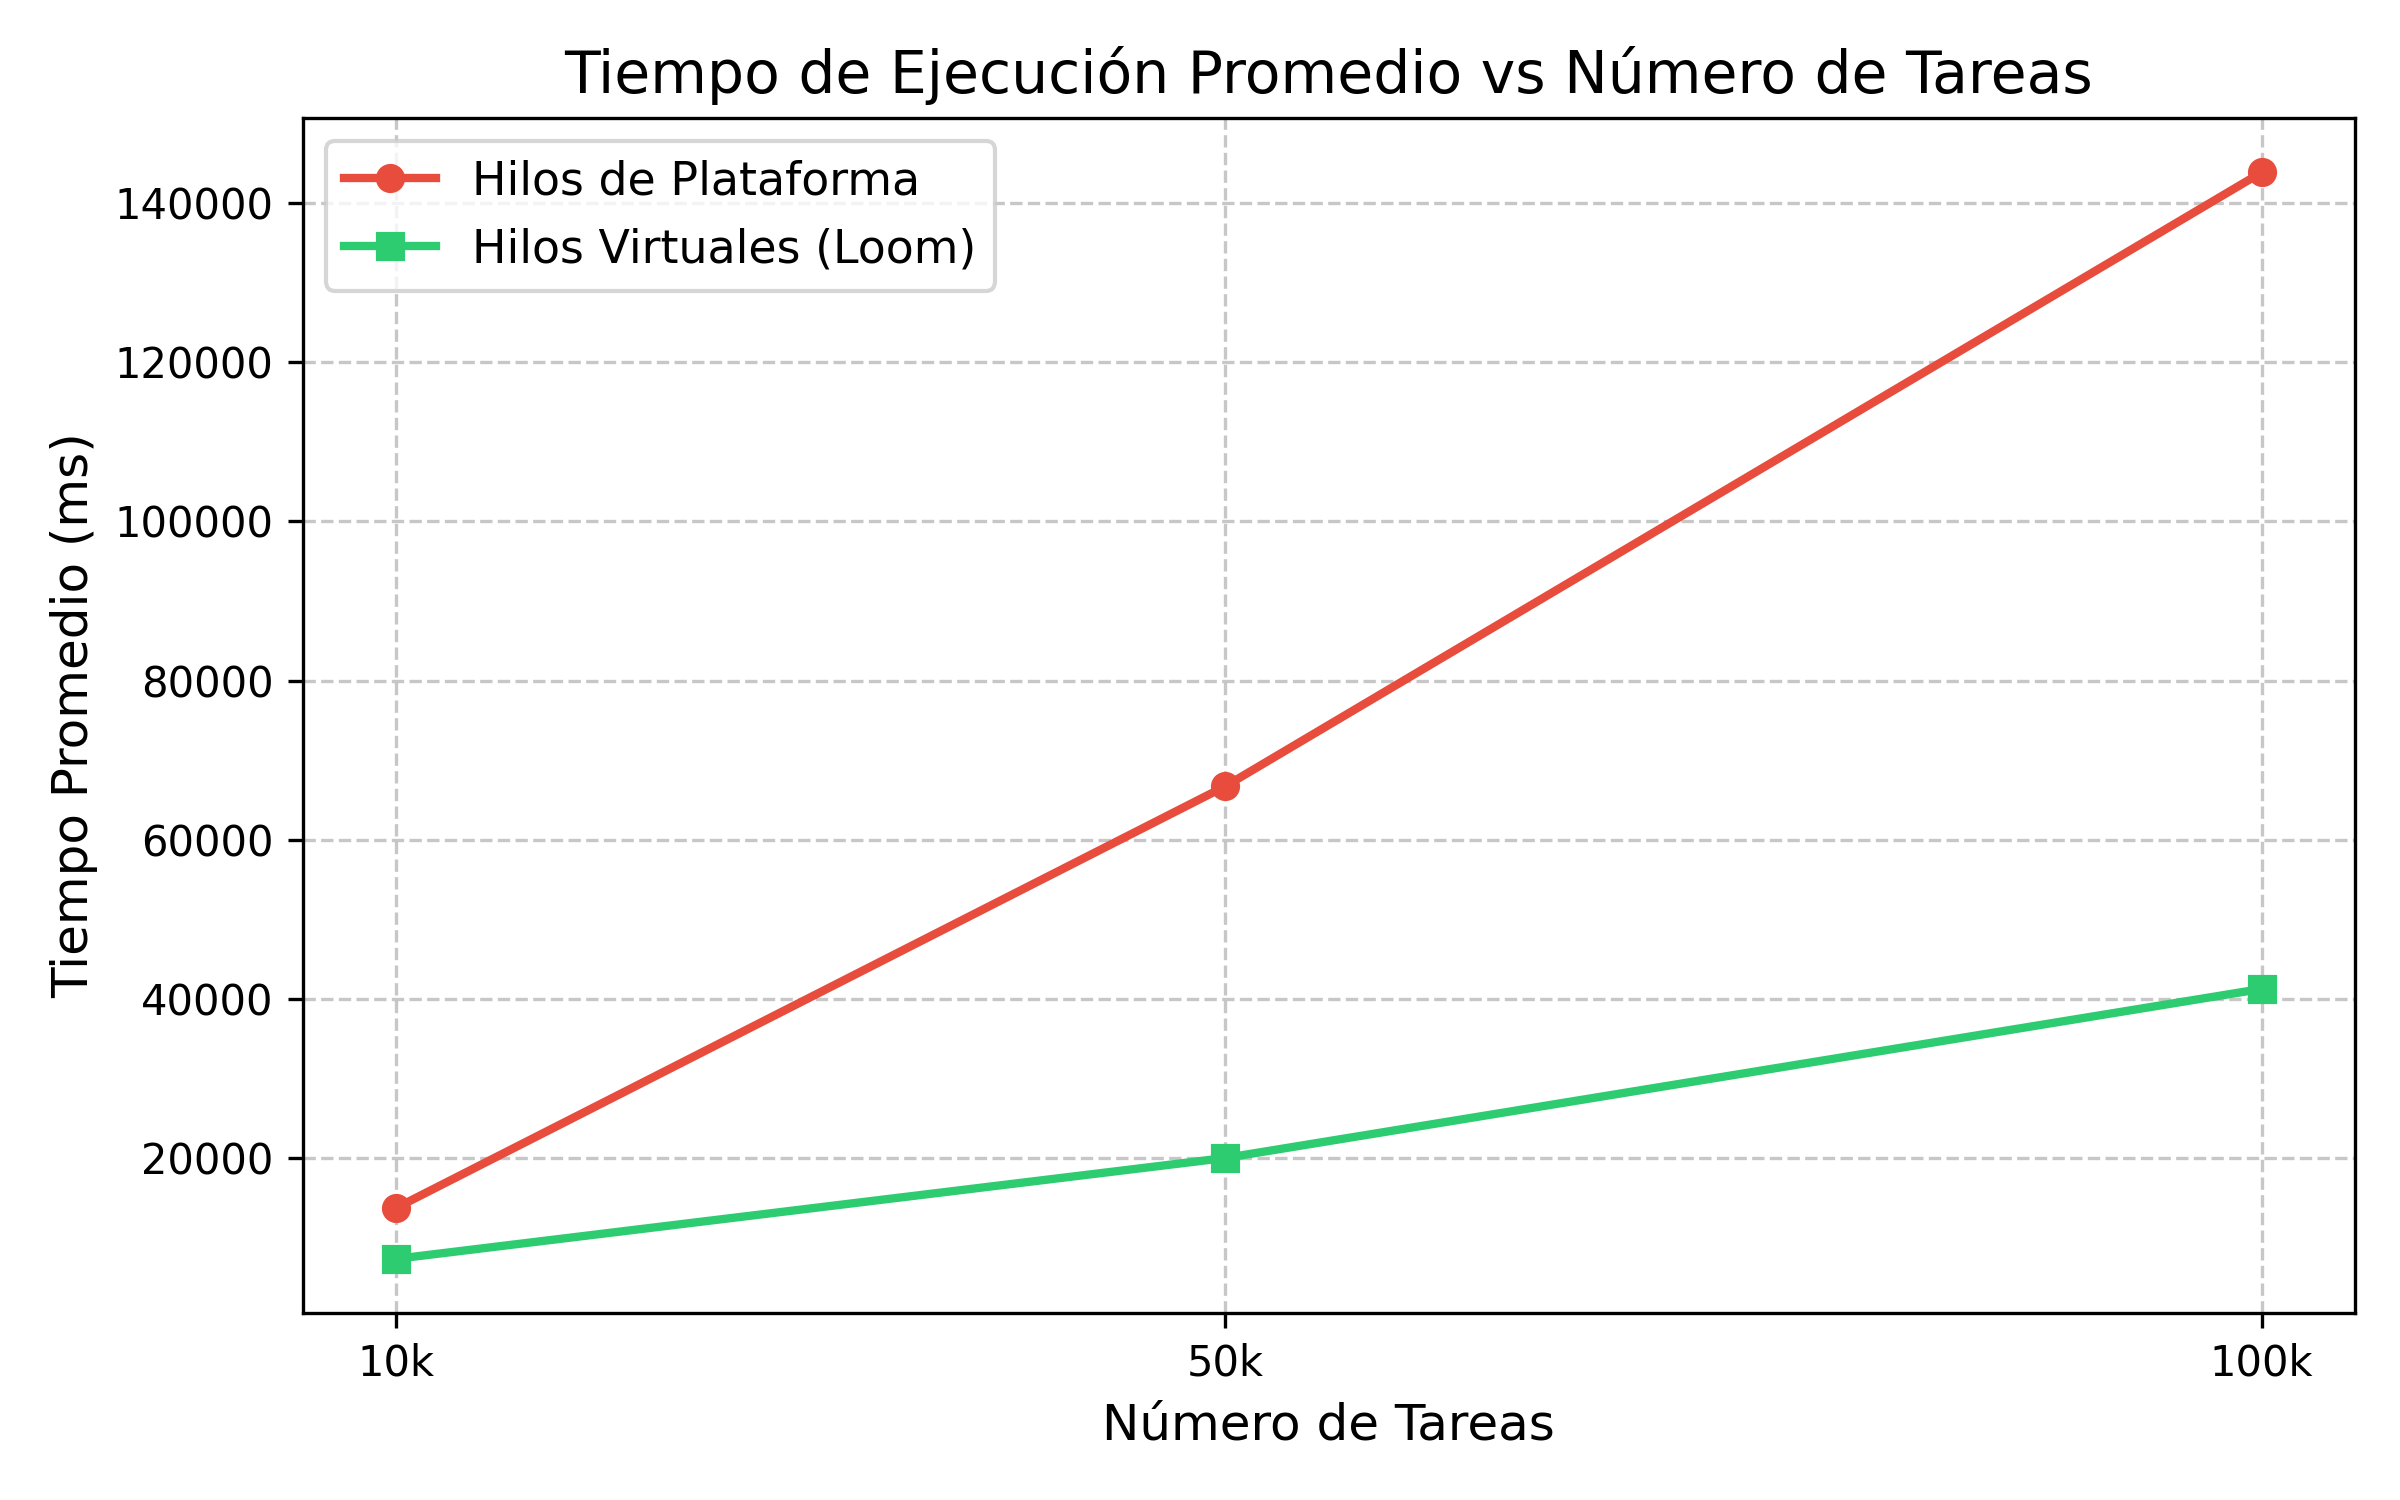
\includegraphics[width=0.8\textwidth]{tiempo_ejecucion_promedio.png}
    \caption{Incremento en el tiempo de ejecución promedio Plataforma vs Hilos Virtuales}
\end{figure}

\begin{figure}[H]
    \centering
    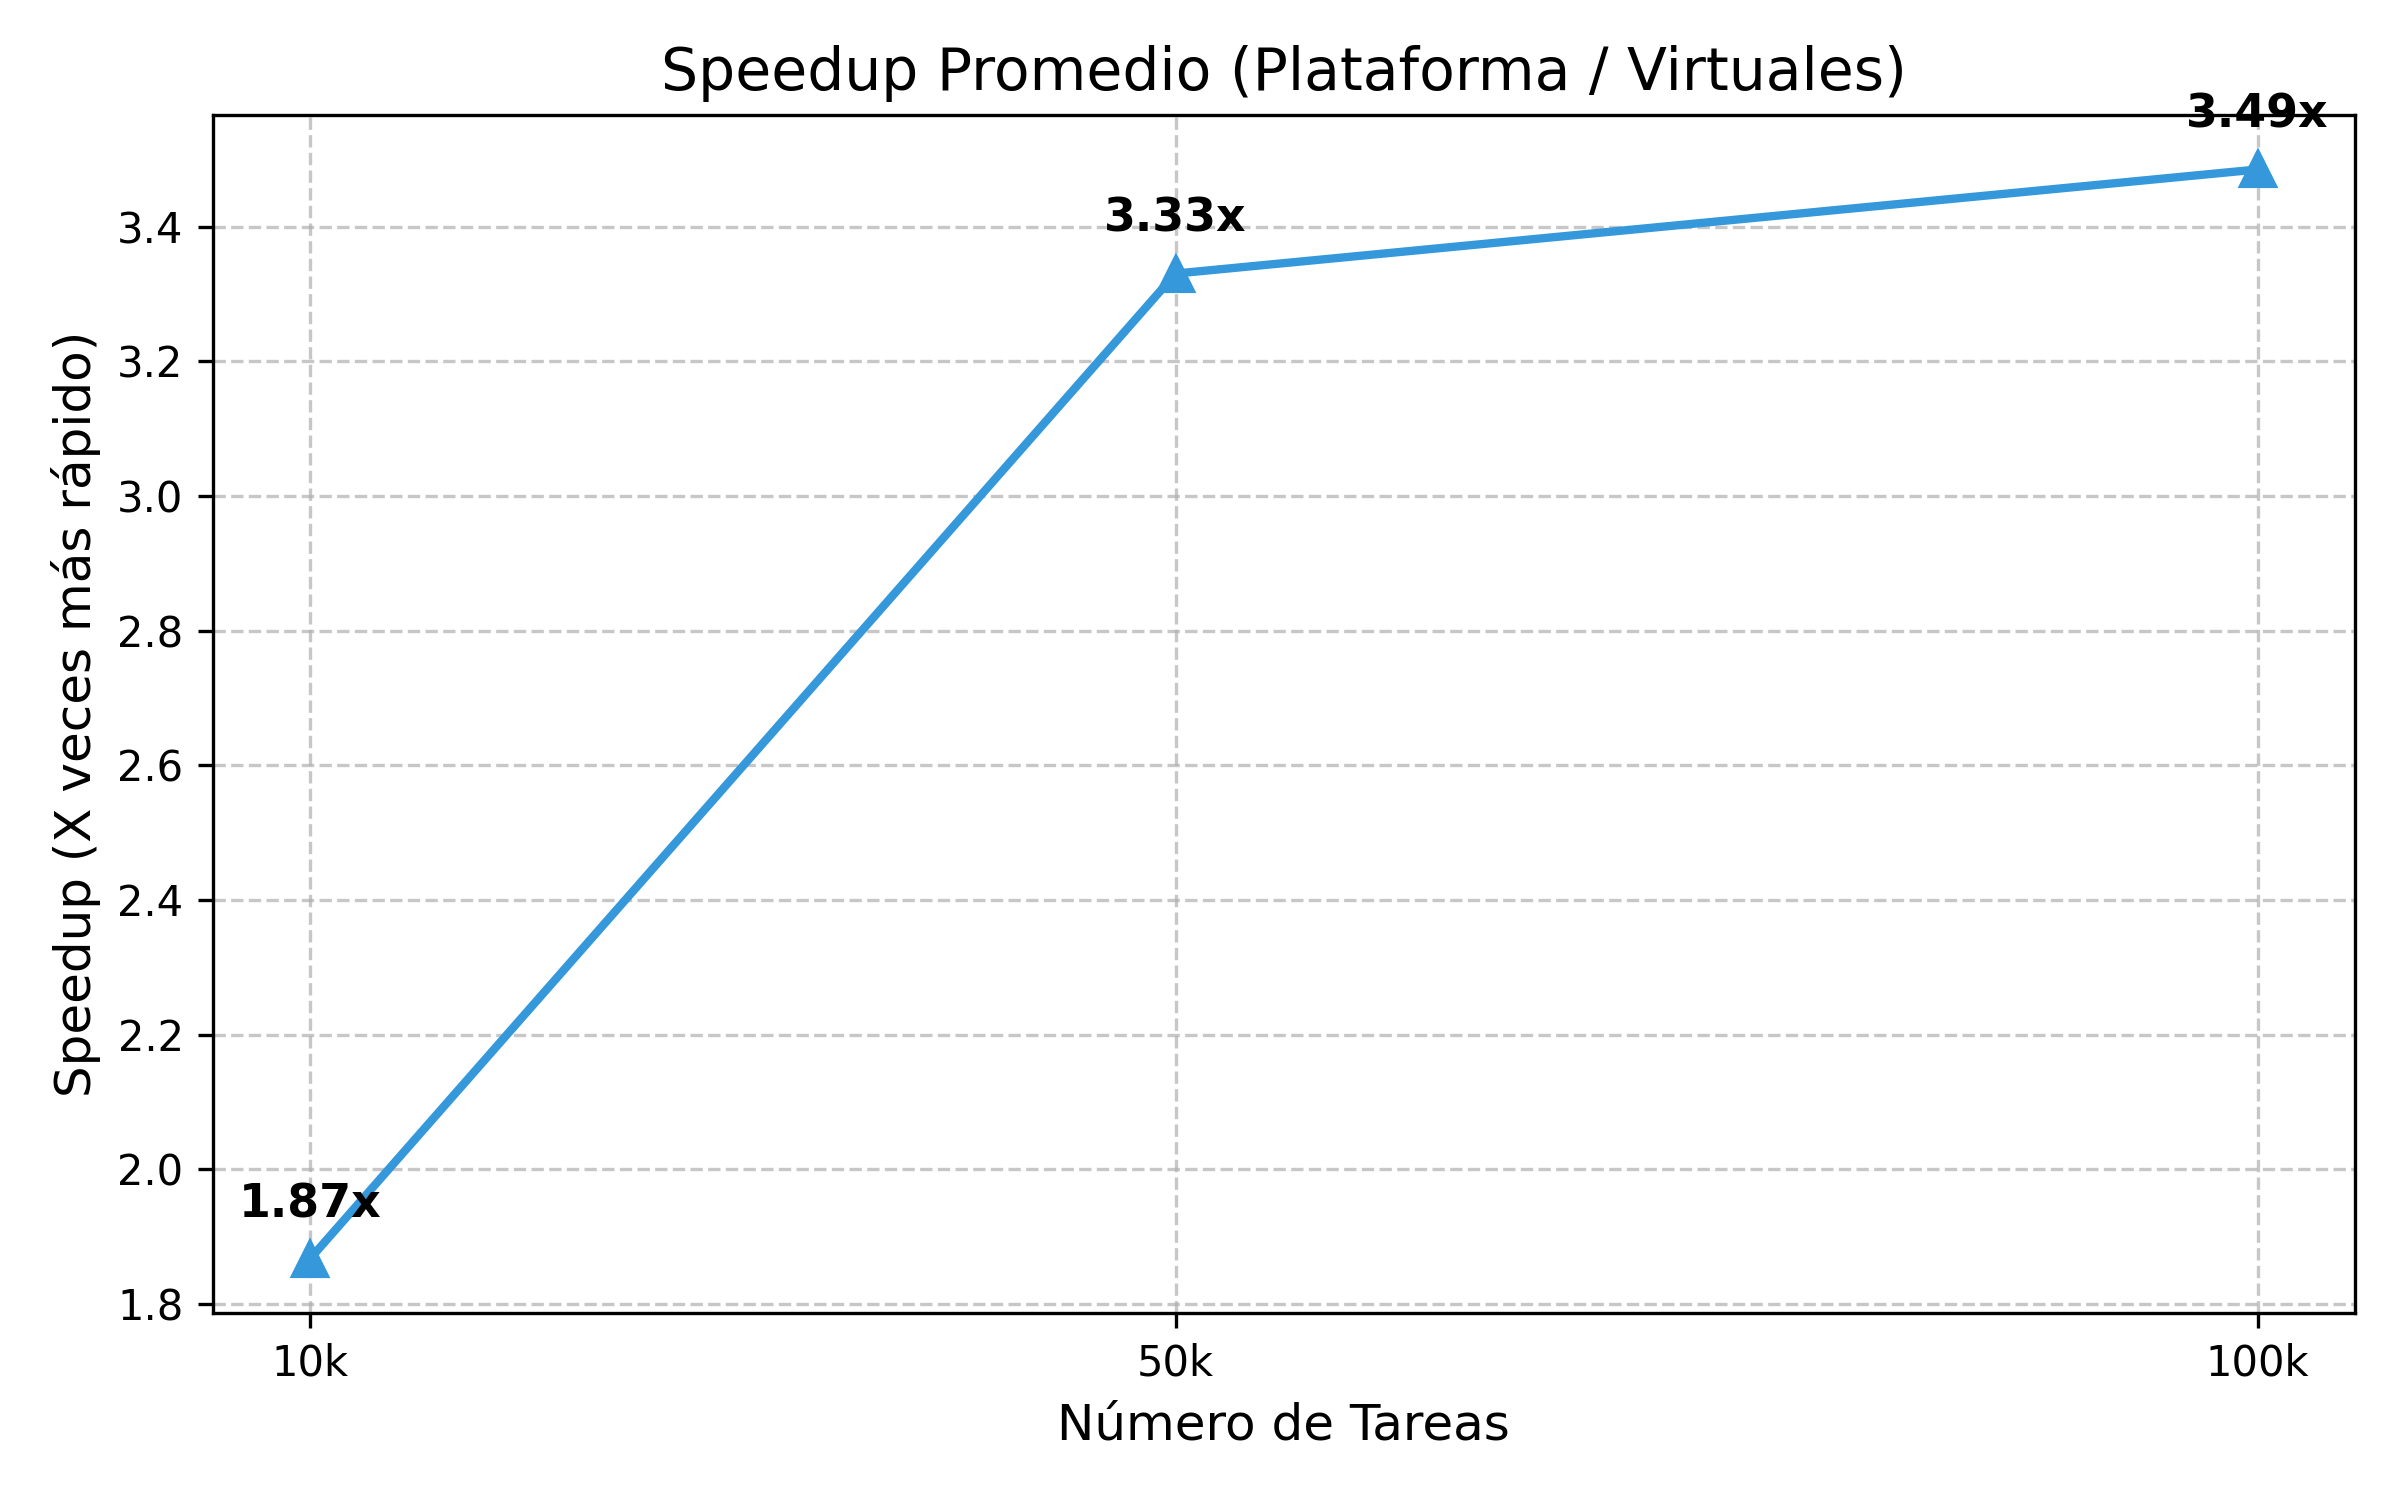
\includegraphics[width=0.8\textwidth]{speedup_promedio.png}
    \caption{Curva de aceleración (Speedup) demostrando escalabilidad ante cargas altas}
\end{figure}

\section{Análisis técnico}

\subsection{Ventajas en escenarios I/O-Bound (Concepto del Carrier Thread)}
Los datos demuestran un \textit{SpeedUp} que escala rápidamente a medida que aumentan las tareas (1.86x para 10k tareas, escalando a 3.48x para 100k tareas). Esta mejora en escenarios I/O-bound (donde hay esperas como el \texttt{Thread.sleep}) se explica por la arquitectura del \textbf{Carrier Thread} (hilo portador).

Cuando la JVM inicia, gestiona un \textit{pool} de hilos reales del SO (16 en la computadora del experimento). Estos son los \textit{Carrier Threads}. Cuando un hilo virtual en la iteración llega a la instrucción de bloqueo (\texttt{sleep}), en lugar de paralizar el núcleo físico del procesador (como ocurre con los hilos de plataforma), la JVM realiza un proceso de desmontaje (\textit{unmounting}). Guarda el estado del hilo virtual en la memoria \textit{heap} y libera al hilo portador \cite{jep444}. El \textit{Carrier Thread} queda inmediatamente libre para ejecutar otra de las 100,000 tareas pendientes. Gracias a esto, Java procesó virtualmente las pausas de las 100,000 tareas de manera simultánea.

\subsection{Comparación con escenarios CPU-Bound}
En contraste, si el experimento se basara en operaciones puramente matemáticas sin tiempos de espera, como cálculos de punto flotante complejos o algoritmos de minería criptográfica, el desempeño de los hilos virtuales sería estadísticamente idéntico, o incluso ligeramente inferior a los de plataforma.
En un escenario CPU-bound, los procesos jamás ceden el control al toparse con un bloqueo. Por ende, un hilo virtual jamás se liberaría. Al no existir hilos disponibles, el \textit{Carrier Thread} se mantiene ocupado al 100\%, saturando rápidamente los núcleos físicos del equipo. La creación de más hilos virtuales solo añadiría una carga innecesaria al planificador (\textit{scheduler}) de la JVM.

\subsection{Relación con la Ley de Amdahl}
La Ley de Amdahl modela los límites de aceleración teórica de los sistemas paralelos basándose en su fracción estrictamente secuencial \cite{amdahl}, y se denota bajo la ecuación:

$$S(s) = \frac{1}{(1 - p) + \frac{p}{s}}$$

Donde $p$ es la porción de código paralelizable y $1-p$ la porción secuencial, lo no paralelizable.
En el experimento realizado, la fase de espera y el filtro de las cadenas de texto conforman la zona paralelizable ($p$). Sin embargo, para evitar la corrupción de datos en los archivos de salida, se utilizó un bloque \texttt{synchronized(writeLock)}. Esto conforma la fracción secuencial ($1-p$).

Aunque los hilos virtuales permitieron que el número de workers ($s$) tendiera hacia 100,000, reduciendo el término $\frac{p}{s}$ casi a cero, el tiempo total de ejecución ($41,274$ ms en promedio para la máxima carga) estuvo dictado por el límite de la Ley de Amdahl: $\frac{1}{1 - p}$. Miles de hilos procesaron sus datos casi de forma instantánea, pero tuvieron que formarse secuencialmente generando un cuello de botella para escribir físicamente en el disco.

\subsection{Diferencias en el consumo de memoria}
La Figura 3 muestra un fenómeno particularmente revelador en la arquitectura propuesta con Loom, una vez aislado el costo del procesamiento de las cadenas de texto.
\begin{figure}[H]
    \centering
    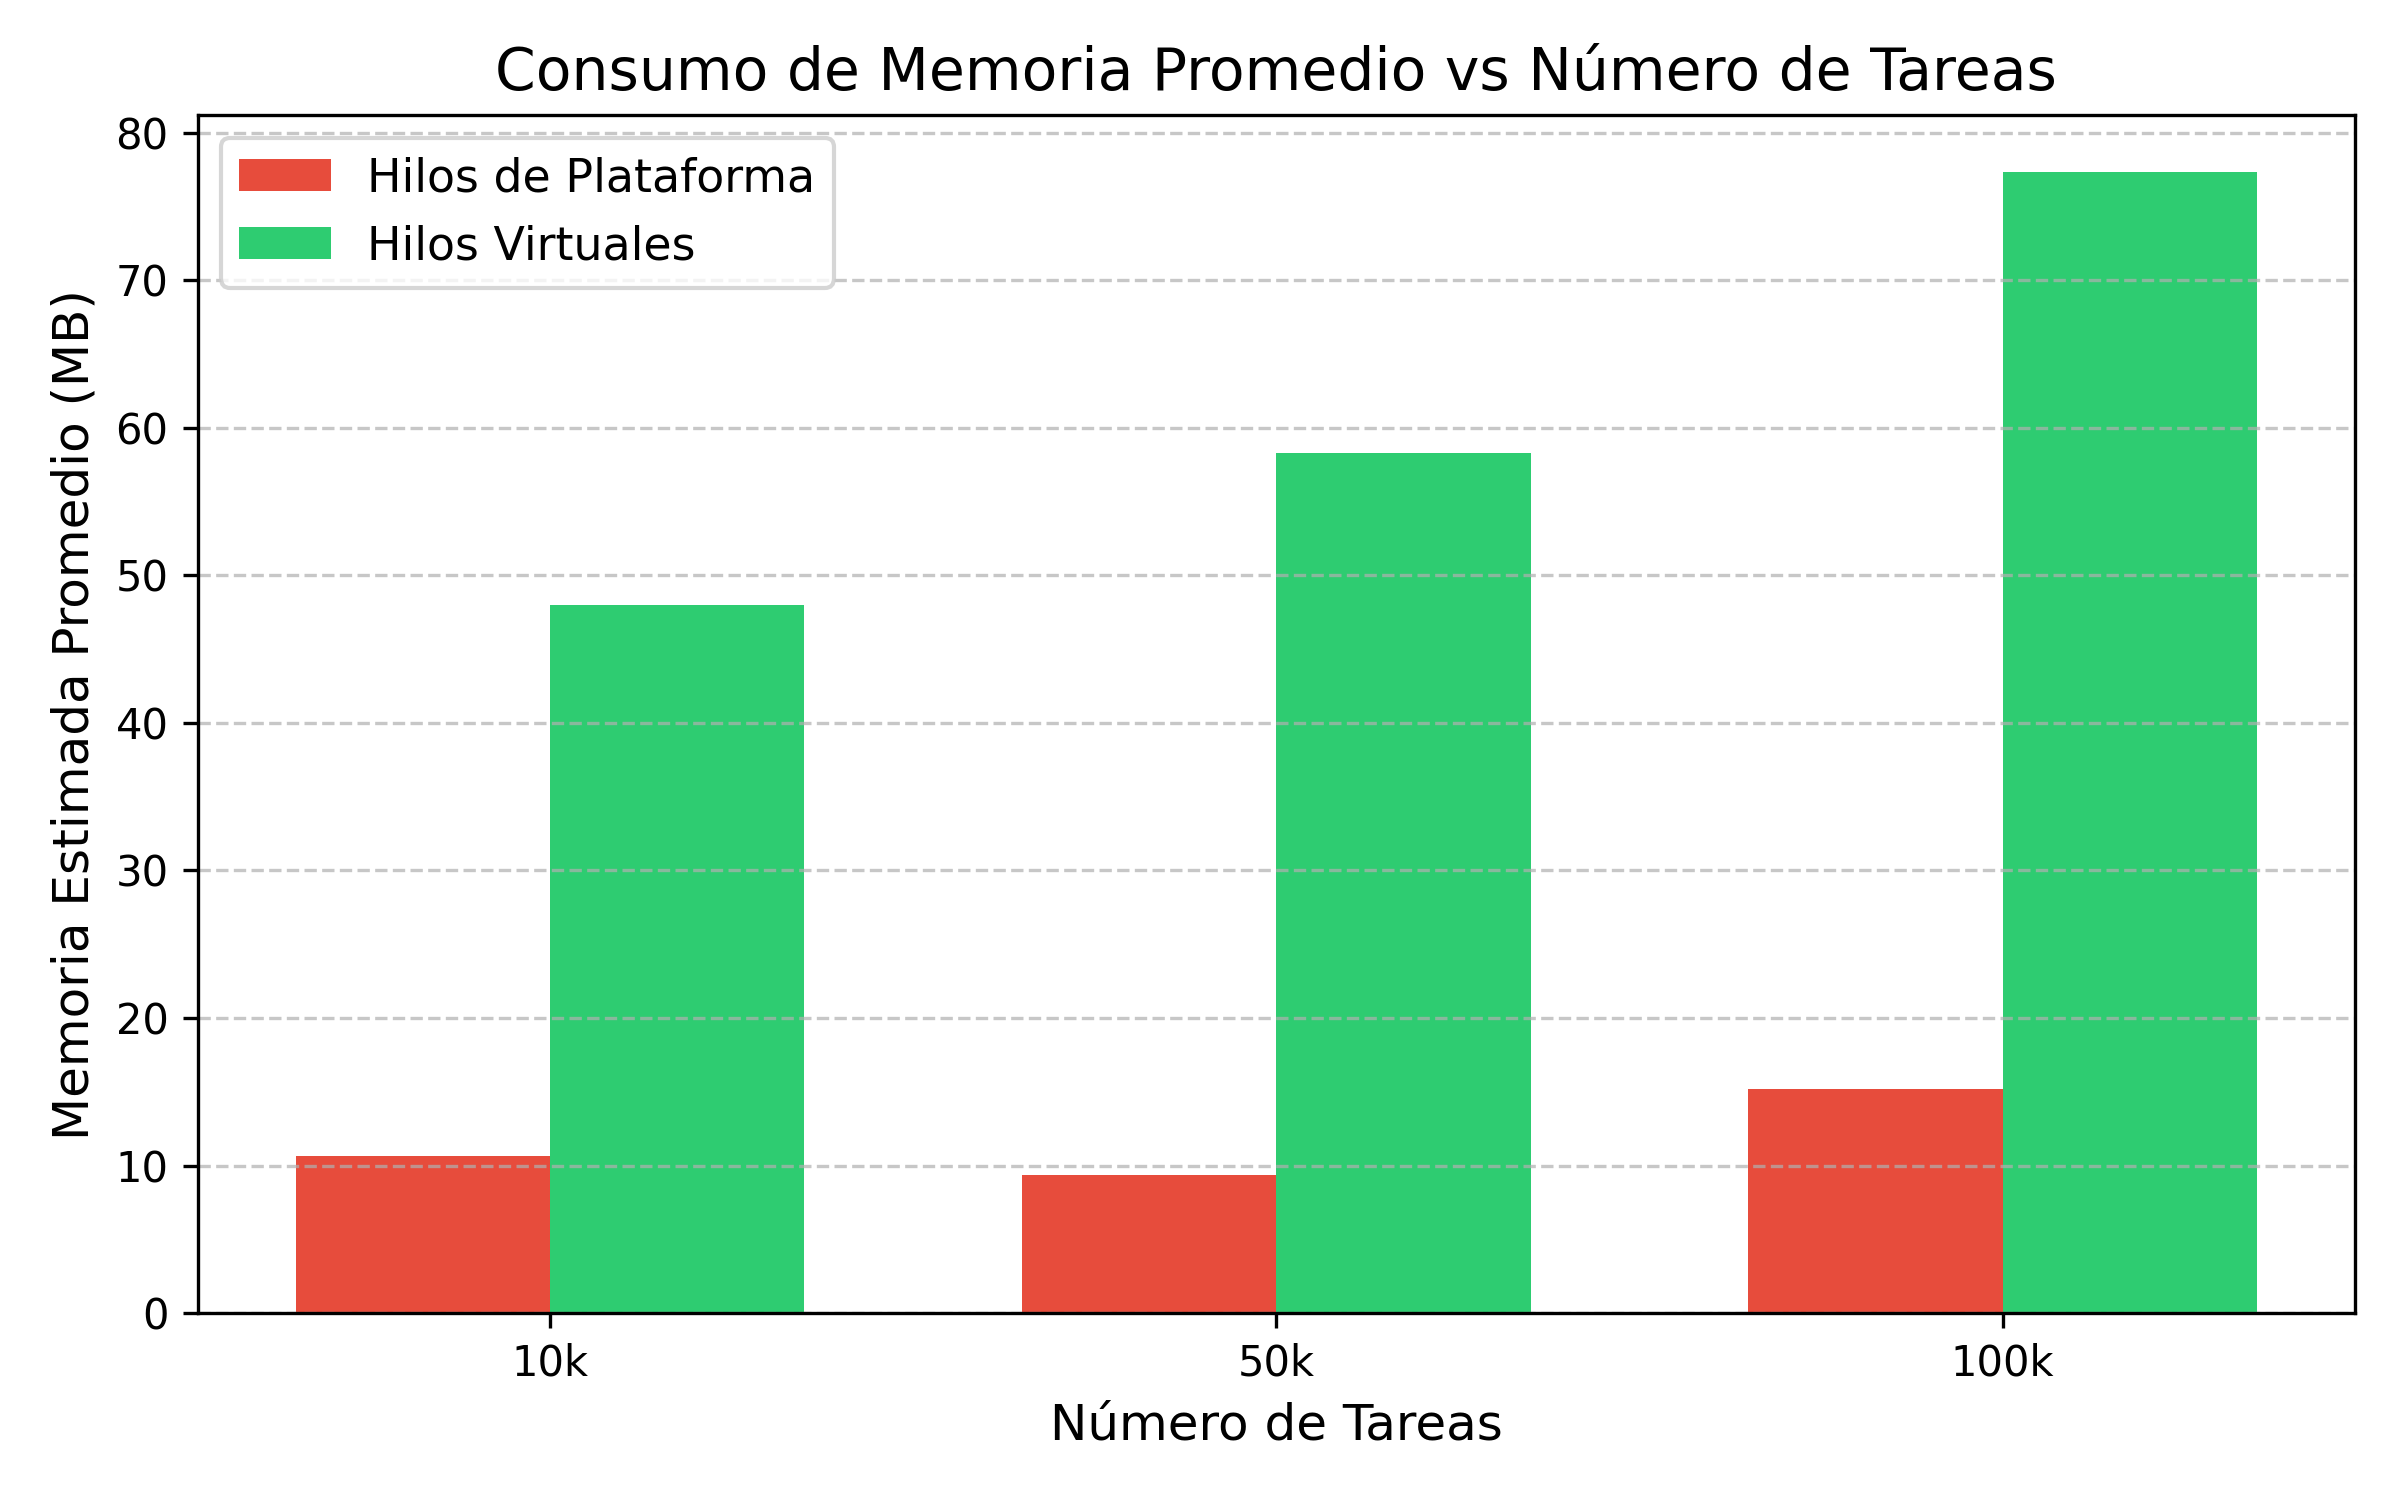
\includegraphics[width=0.8\textwidth]{consumo_memoria_promedio.png}
    \caption{Comparativa de uso en memoria (Heap). Loom aloja 100,000 hilos reales en muy poca memoria.}
\end{figure}
Los hilos de plataforma tradicionales requieren asignar una porción de memoria continua en el \textit{stack} del sistema operativo (configurado por defecto en 1 MB en máquinas virtuales de 64 bits) \cite{oracleTuning}. Para la prueba, debido a esto, no se crearon 100,000 hilos de plataforma (lo que hubiera exigido 100 GB de RAM y ocasionado un desbordamiento de memoria); en su lugar, el gestor utilizó una cola virtual de tareas (\textit{Queue}) de solo $\sim15$ MB en \textit{Heap}, mientras se apoyaba en el \texttt{FixedThreadPool} de 16 hilos.

Por otro lado, el motor Loom instanció directamente las 100,000 entidades virtuales simultáneamente en la zona del \textit{Heap}. Un hilo virtual solo ocupa unos pocos cientos de bytes como metadatos recolectables por el GC \cite{jep444}.
Al dividir el pico máximo de $77.33$ MB registrado en la máxima carga de 100,000 tareas, resulta que cada hilo virtual operó pesando en promedio $\sim770$ bytes por instancia, lo que corrobora la drástica ligereza prometida por Java 21 sobre los hilos convencionales OS de 1 MB.

\section{Conclusiones}
El uso de los Hilos Virtuales de Java 21 (Project Loom) representa un punto de inflexión para arquitecturas concurrentes, superando sin modificar realmente la POO utilizada en el modelo clásico Manager-Worker. 

Los resultados del diseño experimental promediados comprueban que los hilos virtuales ofrecen un desempeño superior en cargas masivas con bloqueos (I/O-bound), con un pico de aceleración comprobado de 3.48x, evitando los graves incrementos de tiempo observados en hilos de plataforma y con un uso de memoria pequeño de apenas cientos de bytes por proceso. No obstante, el experimento también demuestra que no se puede evitar la Ley de Amdahl en operaciones de almacenamiento o recursos compartidos (como la escritura única a disco), concluyendo que los beneficios de Loom encontrarán rápidamente su límite si el diseño de sistemas no contempla separar o mejorar las secciones críticas mutuamente excluyentes del código fuente.

\bibliographystyle{IEEEtran} 
\bibliography{lib}

\end{document}